\subsection{Deep multi-platform RNA sequencing of the Syn1 and Syn3A transcriptomes}

The \syn~and \syna~transcriptomes were sequenced on complementary platforms whose depth, read length, and cross-platform agreement are summarized in Table~\ref{tbl:seq-summary} and Fig.~\ref{fig:si-rnaseq}.
For \syn, PacBio Iso-Seq combined the greatest sequencing depth (4{,}184$\times$ genome-mean) with the longest reads (median 1.56~kb), several-fold longer than the \syn~ONT direct-RNA reads (median 338--458~nt) in Fig.~\ref{fig:si-rnaseq}b, so the full-length PacBio isoforms were selected for operon calling.
Two independent ONT direct-RNA runs of \syn~were performed, yet they agreed only moderately in depth, read length, and per-gene transcript abundance (Pearson $r = 0.82$ on $\log_{10}$ transcripts per million (TPM); Fig.~\ref{fig:si-rnaseq}a), below the nearly unitity $r$ reproducibility of the Illumina and PacBio technical replicates.
Part of this run-to-run variability tracked the different ribosomal-RNA depletion chemistries of the two libraries (Methods), and part the short read length and the pervasive 3$'$ RNA processing described below, together indicating that direct-RNA sequencing of these degradation-prone transcripts would benefit from a dedicated RNA-protection protocol.

The PacBio and Illumina TPM were nonetheless consistent (Pearson $r = 0.62$, in line with previous reports~\cite{yan_smrt-cappable-seq_2018}; Fig.~\ref{fig:si-rnaseq}a), with only a mild over-representation of long and low-abundance transcripts by PacBio (Fig.~\ref{fig:si-rnaseq}c,d).
The two ONT runs correlated with Illumina to a similar degree, whereas the correlation between ONT and PacBio was weaker (Pearson $r = 0.5$).
Illumina TPM was therefore used as the quantitative transcriptome axis for both \syn~and~\syna~throughout, to avoid the bias introduced by different sequencing platforms.

For \syna, only Illumina and ONT direct-RNA sequencing were available, with no PacBio library.
The \syna~ONT reads were short (median 355~nt, similar to the \syn~ONT run 2 with the same protocol), too short to reconstruct full operon structures de novo as the PacBio isoforms did for \syn, but sufficient to test the co-transcription of individual gene pairs, as applied in the genome-reduction analysis below.
The \syna~ONT and Illumina TPM agreed to a degree comparable to the cross-platform comparisons in \syn~(Pearson $r = 0.57$; Fig.~\ref{fig:si-rnaseq}e).

\begin{table}[htbp]
\centering
\caption{Summary of the RNA sequencing libraries for \syn~and \syna.}
\ltbl{seq-summary}
\renewcommand{\arraystretch}{1.2}
\resizebox{\textwidth}{!}{%
\begin{tabular}{l l l l r r r l r}
\toprule
Organism & Platform & Read type & SRA accession(s) & Reads\textsuperscript{b} & Mapped\textsuperscript{b} & Rate & Read length & Depth ($\times$)\textsuperscript{c} \\
\midrule
\syn  & PacBio Iso-Seq (HiFi) & full-length cDNA      & SRR36012641--43 & 2.95~M raw HiFi & 2.60~M\textsuperscript{a} & 88.2\% & median 1.56~kb & 4184 \\
\syn  & Illumina MiSeq        & paired-end 251 cycles/end & SRR35996296--98 & 2.10~M & 2.08~M & 99.2\% & median 212~nt & 766 \\
\syn  & ONT direct RNA        & native RNA, run 1     & SRR36199726 & 234~k & 207~k & 88.5\% & median 458~nt & 116 \\
\syn  & ONT direct RNA        & native RNA, run 2     & SRR36199725 & 585~k & 457~k & 78.1\% & median 338~nt & 127 \\
\syna & Illumina              & paired-end 2$\times$51~nt  & SRR19432056--57~\cite{sandberg_adaptive_2023} & 12.7~M & 12.5~M & 98.3\% & 51~nt & 2355 \\
\syna & ONT direct RNA        & native RNA, 1 run     & SRR36199724 & 734~k & 559~k & 76.2\% & median 355~nt & 313 \\
\bottomrule
\end{tabular}%
}
\par\smallskip
{\footnotesize
\begin{minipage}{\textwidth}
\raggedright
All libraries are strand-specific; the Illumina libraries used the dUTP protocol.\\
\textsuperscript{a}2.60~M high-quality full-length reads retained after quality control (Methods).\\
\textsuperscript{b}Illumina values are read pairs with both mates mapped; PacBio and ONT values are reads (primary alignments), with the PacBio Reads column giving the raw HiFi count.\\
\textsuperscript{c}Genome-mean per-base sequencing depth over both strands (sense $+$ antisense), which, given negligible antisense in this gene-dense genome, approximates the average sense-gene coverage.
% \textsuperscript{d}The \syn~MiSeq reads were deposited 3$'$-adapter-trimmed at demultiplexing and are therefore of variable length (maximum 250~nt, 22.4\% of reads full length), because the library inserts are shorter than the read; the \syna~reads are untrimmed and uniformly 51~nt (Methods).
\end{minipage}}
\end{table}

\begin{sifigure}[htbp]
\centering
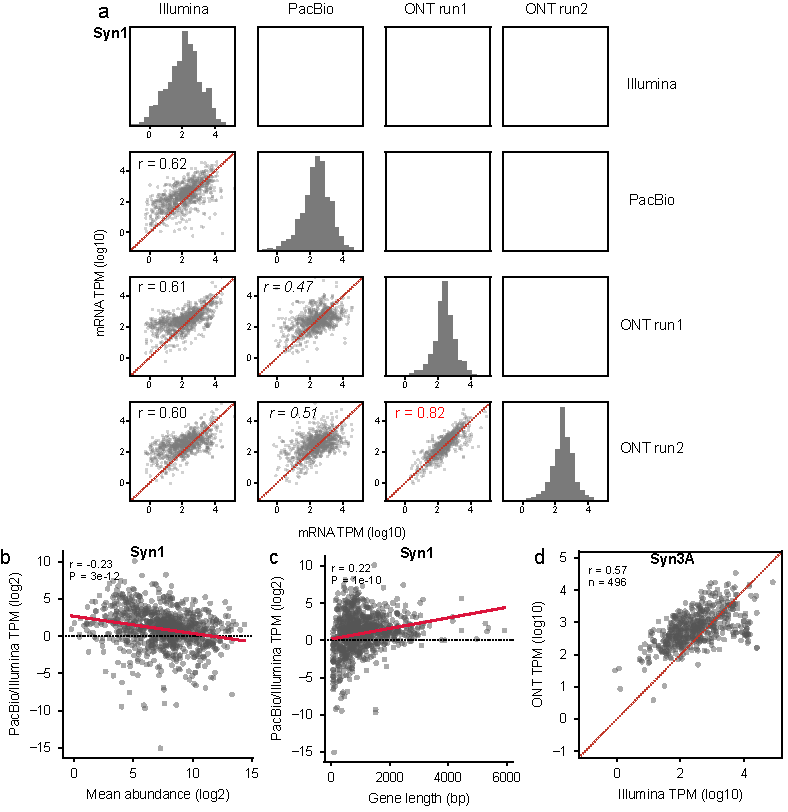
\includegraphics[scale=1]{figures/si-rnaseq.pdf}
\caption{\textbf{Cross-platform and cross-run comparison of RNA-seq quantification.}
\textbf{(a)} \syn~per-gene mRNA TPM across Illumina, PacBio, and the two ONT runs, in that order along both axes: lower triangle, pairwise $\log_{10}$--$\log_{10}$ scatter with the identity line; diagonal, per-platform $\log_{10}$ TPM distribution.
\textbf{(b)} \syn~mapped-read length distribution for each platform (Illumina, PacBio, ONT run 1, ONT run 2; top to bottom) on a shared axis, with the median marked; short-read Illumina, intermediate ONT, and long-read PacBio occupy distinct length regimes.
\textbf{(c)} \syn~gene-length dependence of the PacBio-to-Illumina TPM ratio, with a linear fit.
\textbf{(d)} The same ratio against mean $\log_{2}$ abundance.
\textbf{(e)} \syna~ONT versus Illumina~\cite{sandberg_adaptive_2023} TPM ($\log_{10}$--$\log_{10}$).}
\lfig{si-rnaseq}
\end{sifigure}
